\documentclass{book}

\usepackage{much_style}


%Командаы 
\newcommand{\newbeggining}[5]{
\vspace{1,8cm}

\section*{#1} \addcontentsline{toc}{section}{\textbf{#2} \newline #1}
\textit{#2} \footnote[1]{#3}

{\small \textbf{Аннотация. }#4

\textbf{Ключевые слова: }#5}
\fancyhead[LO]{\small #2}
\fancyhead[RE]{\small #2}
\fancyhead[RO]{\thepage}
\fancyhead[LE]{\thepage}
\index{#2}

\setcounter{section}{0}
\setcounter{theorem}{0}
\setcounter{figure}{0}
\setcounter{table}{0}
\setcounter{equation}{0}
}


\newcommand{\begginingdouble}[7]{
\vspace{1.8cm}
\setcounter{section}{0}
\setcounter{theorem}{0}
\setcounter{figure}{0}
\setcounter{table}{0}
\setcounter{equation}{0}



\section*{#1} \addcontentsline{toc}{section}{\textbf{#2, #4} \newline #1}
\textit{#2\footnote[1]{#3}, #4\footnote[7]{#5}}
\index{#2}
\index{#4}\par
{\small \textbf{Аннотация. }#6

\textbf{Ключевые слова: }#7}
\fancyhead[LO]{\small #2}
\fancyhead[RE]{\small #2}
\fancyhead[RO]{\thepage}
\fancyhead[LE]{\thepage}
}
%

%вручную писать библиографию не через файл
%аннотацию
%выводит емайл
%счётчик таблиц рисунков
%авторский указатель
% колонтитул заголовок автор
%два автора?-отдельная коммманда
%
\begin{document}



%==Титульная страница
\thispagestyle{empty}
\begin{center}
Министерство науки и высшего образования Российской Федерации\\
Федеральное государственное бюджетное образовательное\\
учреждение высшего образования\\
<<Иркутский государственный университет>>\\
(ФГБОУ ВО <<ИГУ>>)
\end{center}

\vspace{3.5cm}

\begin{center}
{\bf 
СБОРНИК СТАТЕЙ\\[1mm]
}  

\vspace{0.3cm}

{
Материалы международной конференции\\[1mm]

} %Текст должен быть набран ЗАГЛАВНЫМИ БУКВАМИ
\end{center}



%Вторая страница
\vfill 
\noindent
\begin{minipage}{\textwidth}
\centering	 Иркутск, 2022
\end{minipage}
\newpage
%==Титульная страница
\thispagestyle{empty}
\begin{center}
Печатается по разрешению редакционно-издательского совета\\
Иркутского государственного педагогического университета

\end{center}

УДК 512.7+121-564.7

ББК 23.42+25.21-23.12
\vspace{1.5cm}



\textbf{Сборник статей. Материалы международной конференции.} --- Иркутск, издательство ГОУ ВПО <<Иркутский государственный педагогический университет>>, 2004.--- 28с.

\vspace{4.3cm}
\textbf{Редакционная коллегия:}

\setlength{\leftskip}{1.5cm}
студент гр. 2471 Толкачев Г.А. 

\setlength{\leftskip}{0pt}


%Содержание
\newpage
\renewcommand{\contentsname}{Содержание}
\noindent\tableofcontents
\thispagestyle{empty}
\newpage\null\thispagestyle{empty}\newpage


\newbeggining{Теория чисел}{Бухштаб А. А.}{example@mail.com}{Способы разложения числа e в цепную дробь путём приведения числа к уровнению пределов.}{Теория чисел, дробь, цепная дробь.}

\begin{center}
	\textbf{Разложение числа $e$ в цепную дробь}
\end{center}
В качестве примера рассмотрим разложение в цепную дробь числа $e$.
\setcounter{equation}{13}
\begin{theorem}
	$$
	\frac{e+1}{e-1}=2+\sqrt[1]{6}+\sqrt[1]{10}+\ldots+\sqrt[1]{4n+2}+\ldots
	$$
\end{theorem}
\begin{proof}
	Определим $f_{n}(x)\ (n=0,\ 1,\ 2,\ \ldots)$ как сумму ряда:
\begin{multline*}
f_{n}(x)=\frac{n!}{(2n)!}+\frac{(n+1)!}{1!(2n+2)!}x^{2}+\frac{(n+2)!}{2!(2n+4)!}x^{4}+\ldots=\\=\sum\limits_{s=0}^{\infty}\frac{(n+s)!}{s!{2n+2s}!}x^{2s}.
\end{multline*}
	Этот ряд сходится при любых значениях $x$; однако мы будем рассматривать только значение $x$, лежащие в интервале $(0; 1)$.
\end{proof}
Легко проверить что имеет место тождество 
\begin{equation}\label{eq1} 
	f_{n}(x)-(4n+2)f_{n+1}(x)=4x^{2}f_{n+2}(x).
\end{equation}
Действительно, коэффициент при $x^{2k}$ в левой части равенства \eqref{eq1} равен
		\begin{gather*}
		\frac{(n+k)!}{k!(2n+2k)!}-(4n+2)\frac{(n+k+1)!}{k!(2n+2k+2)!}=\\
		=\frac{(n+k)!}{k!(2n+2k)!}(1-\frac{2n+1}{2n+2k+1})=\frac{2(n+k)!}{(k-1)!(2n+2k+1)!}.
		\end{gather*}
а в правой части равенства \eqref{eq1} он равен
\begin{equation*}
	\frac{4(n+k+1)!}{(k-1)!(2n+2k+2)!}=\frac{2(n+k)!}{(k-1)!(2n+2k+1)!}
\end{equation*}
так что \eqref{eq1} верно.
Обозначим $\dfrac{f_{n}(\frac{1}{2})}{f_{n+2}(\frac{1}{2})}$ через $a_{n}$. В частности, поскольку
\begin{equation*}
	f_{0}(x)=1+\frac{x^{2}}{2!}+\frac{x^{4}}{4!}+\ldots=\frac{1}{2}(e^{x}+e^{-x})
\end{equation*}
\begin{equation*}
	f_{1}(x)=\frac{1}{2x}+(x+\frac{x^{3}}{3!}+\frac{x^{5}}{5!}+\ldots)=\frac{1}{4x}(e^{x}-e^{-x}).
\end{equation*}
то
\begin{equation*}
	\alpha_{0}=\frac{f_{0}(\frac{1}{2})}{f_{1}(\frac{1}{2})}=\frac{e^{\frac{1}{2}}+e^{-\frac{1}{2}}}{e^\frac{1}{2}-e^{-\frac{1}{2}}}=\frac{e+1}{e-1}
\end{equation*}
Из тожественного равенства \eqref{eq1} при $x=\frac{1}{2}$ получаем:
\begin{equation} \label{eq2} 
	\alpha=(4n+2)+\frac{1}{\alpha_{n+1}}. 
\end{equation}
Поскольку $\alpha_{n+1}$ положительно, равенство \eqref{eq2} показывает, что при всех $n$ $\alpha_{n}>4n+2>1,\dfrac{1}{\alpha_{n+1}}<1$ т.е. $4n+2=[\alpha_{n}]$ и последовательность отношений \eqref{eq2} при $n=0,1,2\ldots$
\begin{equation*}
	\begin{split}
		\alpha_{0}&=\ 2+\frac{1}{\alpha_{1}}\\
		\alpha_{1}&=\ 6+\frac{1}{\alpha_{2}}\\
		\alpha_{2}&=10+\frac{1}{\alpha_{3}}\\
		&\dotsb\dotsb\dotsb
		\end{split}
\end{equation*}
даёт разложение $\alpha_{0}$ в цепную дробь:
\begin{equation}\label{eq3}
	\frac{e+1}{e-1}=\alpha_{0}=2+\sqrt[1]{6}+\sqrt[1]{10}+\ldots+\sqrt[1]{4n+2}+\ldots
\end{equation}
\begin{theorem}
	\begin{equation}
	e=2+\sqrt[1]{1}+\sqrt[1]{2}+\sqrt[1]{1}+\sqrt[1]{1}+\sqrt[1]{1}+\sqrt[1]{4}+\sqrt[1]{1}+\sqrt[1]{6}+\ldots \label{eq44}
\end{equation}
	т.е. элемент $\alpha_{n}$ разложения $e$ в цепную дробь	имеют вид:
	\begin{equation*}
		\alpha_{0}=2,\alpha_{3n}=\alpha_{3n+1}=1\text{и} \alpha_{3n-1}=2n 
	\end{equation*}
\end{theorem}
\begin{proof}
	Обозначим подходящие дроби к правой части \eqref{eq44} через $\frac{P_{n}}{Q_{n}}$, а подходящие дроби к \eqref{eq3} через $\frac{R_{n}}{S_{n}}(n=0,1,2,\ldots)$. Докажем, что
	\begin{equation*}
		\frac{R_{n}}{S_{n}}=\frac{P_{3n+1}+Q_{3n+1}}{P_{3n+1}-Q_{3n+1}}.
	\end{equation*}
Принимая во внимание значение элементов цепной дроби \eqref{eq44}, имеем: %почему тут 2?
\begin{equation*}
	\begin{split}
		P_{3n+1}&=P_{3n}+P_{3n-1},P_{3n}=P_{3n-1}+P_{3n-2},\\
		P_{3n-1}&=2nP_{3n-2}+P_{3n+3},\\
		P_{3n-2}&=P_{3n-3}+P_{3n-4}, P_{3n-3}=P_{3n-4}+P_{3n-5},
	\end{split}
\end{equation*}
откуда находим:
\begin{equation*}
	\begin{split}
		P_{3n+1}=2P_{5n-1}+P_{3n+-2}=(4n+1)P_{3n-2}+2P_{3n-3}=\\
		=(4n+2)P_{3n-2}+P_{8n-3}-P_{8n-4}=(4n+2)P_{8n-2}+P_{3n-5}.
	\end{split}
\end{equation*}
\end{proof}
Аналогичное соотношение имеем и для $Q_{3n+1}$, так что
\begin{equation} \label{eq5}
	\begin{rcases*}
		P_{3n+1}=(4n+2)P_{3n-2}+P_{3n-5} \\
		Q_{3n+1}=(4n+2)Q_{3n-2}+Q_{3n-5}
	\end{rcases*} 
\end{equation}
Докажем индукцией по $n$, что
\begin{equation}\label{eq6}
	R_{n}=\frac{1}{2}(P_{3n+1}+Q_{3n+1}).
\end{equation}
Из \eqref{eq3} и \eqref{eq44} непосредственно вычисляем $R_{0}=2,R_{1}=13,P_{1}=3,P_{4}=19,Q_{1}=1,Q_{4}=7$, так что соотношение \eqref{eq6} верно для всех $R$ с номерами, меньшими чем n, где $n\geqslant2$ т.е., в частности,
\begin{equation*}
R_{n}=(4n+2)R_{n-1}+R_{n-2}=\frac{1}{2}\{(4n+2)(P_{3n-5}+Q_{3n-5}) \};
\end{equation*}
тогда, используя равенство \eqref{eq5}, получаем:
\begin{equation*}
	\begin{split}
		R_{n}=(4n&+2)R_{n-1}+R_{n-2}=\frac{1}{2}\{(4n+2)(P_{3n-2}+Q_{3n-2})+
		\\&+P_{3n-5}+Q_{3n-5}\}=\frac{1}{2}(P_{3n+1}+P_{3n+1}).
	\end{split}
\end{equation*}
Согласно принципу полной математической индукции равенство \eqref{eq6} верно для всех $n$.
Совершенно аналогично доказывается, что
$$
S_{n}=\frac{1}{2}(P_{3n+1}-Q_{3n-1}).
$$
Рассмотрим теперь предел отношений величин $R_{n}$ и $S_{n}$, находим:
\begin{equation*}
	\frac{\lim\limits_{n\to\infty}\dfrac{P_{3n+1}}{Q_{3n+1}}+1}{\lim\limits_{n\to\infty}\dfrac{P_{3n+1}}{Q_{3n+1}}-1}=\lim\limits_{n\to\infty}\frac{P_{3n+1}+Q_{3n+1}}{P_{3n+1}-Q_{3n+1}}=\lim\limits_{n\to\infty} \frac{R_{n}}{S_{n}}=\frac{e+1}{e-1}
\end{equation*}
т.е.
$$
\lim\limits_{n\to\infty}\frac{P_{3n+1}}{Q_{3n+1}}=e.
$$
Поскольку цепная дробь в правой части \eqref{eq44} сходится, мы будем иметь также, что вообще $\lim\limits_{n\to\infty}\dfrac{P_{n}}{Q_{n}}=e$, а это доказывает теорему.

\begin{thebibliography}{1}
\bibitem{Sulsky1994}
Бухштаб, А. А. Теория чисел / А. А. Бухштаб. — Москва : ПРОСВЕЩЕНИЕ, 1966. ---387 с.
\end{thebibliography}



%AAAAAAAAAAAAAAAAAAAAAAAAAAAAAAAAAAAAAAAAAAAAAAAAAAAAAAAAAAAA



\newbeggining{Пирамидальная сортировка} {Уильямс Дж.}{example@mail.com}{На основе исходных данных строится двоичная куча, в которой последовательно собираются минимальные значения}{Сортировка}

\emph{Пирамидальная сортировка} --- алгоритм сортировки, работающий в худшем, в среднем и в лучшем случае (то есть гарантированно) за $O(n\log n)$ операций при сортировке $n$ элементов. Количество применяемой служебной памяти не зависит от размера массива (то есть, $O(1)$).\par
Может рассматриваться как усовершенствованная сортировка пузырьком, в которой элемент всплывает (min-heap) / тонет (max-heap) по многим путям.



\section*{Алгоритм}
Сортировка пирамидой использует бинарное сортирующее дерево. Сортирующее дерево — это такое дерево, у которого выполнены условия:
\begin{wrapfigure}{r}{6.5cm}

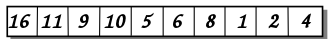
\includegraphics[width=0.5\textwidth]{pics/333px-Сортирующее_дерево_развернутое_в_массив.svg.png}
\caption{Cтруктура хранения данных сортирующего дерева}
\end{wrapfigure}

\begin{enumerate}

    \item[1] Каждый лист имеет глубину либо $d$, либо $d-1$, $d$ --- максимальная глубина дерева.
    \item[2] Значение в любой вершине не меньше (другой вариант — не больше) значения её потомков.
\end{enumerate}


\begin{figure}[h]

\centering
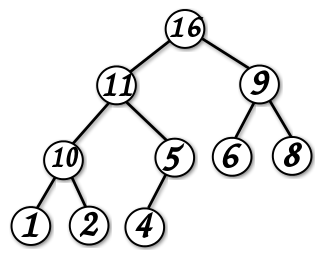
\includegraphics[width=0.5\textwidth]{pics/333px-Сортирующее_дерево.svg.png}
\caption{Пример сортирующего дерева}
\end{figure}

Алгоритм сортировки будет состоять из двух основных шагов:
\begin{enumerate}

    \item[1] Выстраиваем элементы массива в виде сортирующего дерева.\par
    $Array[i]\geqslant Array[2i+1]$\par
    $Array[i]$ и $Array[2i+2]$.\par
    При $0\leqslant i \leqslant n/2$\par
    Этот шаг требует $O(n)$ операций.
    \item[2]  Будем удалять элементы из корня по одному за раз и перестраивать дерево. То есть на первом шаге обмениваем $Array[0]$ и $Array[n-1]$, преобразовываем $Array[0]$, $Array[1],\ldots , Array[n-2]$ в сортирующее дерево. Затем переставляем $Array[0]$ и\linebreak $Array[n-2]$, преобразовываем $Array[0],\ldots, Array[n-3]$ в сортирующее дерево. Процесс продолжается до тех пор, пока в сортирующем дереве не останется один элемент. Тогда $Array[0]$, $Array[1]$, $\ldots$, $Array[n-1]$ --- упорядоченная последовательность.
\end{enumerate}
Этот шаг требует $O(n\log n)$ операций.




\section*{Достоинства и недостатки}
\subsection*{Достоинства}
\begin{itemize}
    \item Имеет доказанную оценку худшего случая $O(n\cdot \log n)$.
    \item Сортирует на месте, то есть требует всего $O(1)$ дополнительной памяти (если дерево организовывать так, как показано выше).
\end{itemize}
\subsection*{Недостатки}
\begin{itemize}
    \item Неустойчив — для обеспечения устойчивости нужно расширять ключ.
    \item На почти отсортированных массивах работает столь же долго, как и на хаотических данных.
    \item На одном шаге выборку приходится делать хаотично по всей длине массива --- поэтому алгоритм плохо сочетается с кэшированием и подкачкой памяти.
    \item Методу требуется <<мгновенный>> прямой доступ; не работает на связанных списках и других структурах памяти последовательного доступа.
    \item Не распараллеливается.
\end{itemize}



\section*{Код}
\subsection*{Java}
\begin{lstlisting}[language=Java, caption={Пирамидальная сортировка на Java}]  
public class HeapSort
{
    public void sort(int arr[])
    {
        int n = arr.length;
        for (int i = n / 2 - 1; i >= 0; i--)
            heapify(arr, n, i);
        for (int i=n-1; i>=0; i--)
        {
            int temp = arr[0];
            arr[0] = arr[i];
            arr[i] = temp;
            heapify(arr, i, 0);
        }
    }
     void heapify(int arr[], int n, int i)
    {
        int largest = i; 
        int l = 2*i + 1; 
        int r = 2*i + 2; 

        if (l < n && arr[l] > arr[largest])
            largest = l;
        if (r < n && arr[r] > arr[largest])
            largest = r;
        if (largest != i)
        {
            int swap = arr[i];
            arr[i] = arr[largest];
            arr[largest] = swap;
            heapify(arr, n, largest);
        }
    }

    static void printArray(int arr[])
    {
        int n = arr.length;
        for (int i=0; i<n; ++i)
            System.out.print(arr[i]+" ");
        System.out.println();
    }

    public static void main(String args[])
    {
        int arr[] = {12, 11, 13, 5, 6, 7};
        int n = arr.length;
        HeapSort ob = new HeapSort();
        ob.sort(arr);
        System.out.println("Sorted array is");
        printArray(arr);
    }
}
\end{lstlisting}
\subsection*{C++}

\begin{lstlisting}[language=C++, caption={Пирамидальная сортировка на C++}]  
#include <iostream>
using namespace std;

void heapify(int arr[], int n, int i)
{
    int largest = i;   
    int l = 2*i + 1;
    int r = 2*i + 2;
    if (l < n && arr[l] > arr[largest])
        largest = l;
    if (r < n && arr[r] > arr[largest])
        largest = r;
    if (largest != i)
    {
        swap(arr[i], arr[largest]);
        heapify(arr, n, largest);
    }
}
void heapSort(int arr[], int n)
{
    for (int i = n / 2 - 1; i >= 0; i--)
        heapify(arr, n, i);
    for (int i=n-1; i>=0; i--)
    {
        swap(arr[0], arr[i]);
        heapify(arr, i, 0);
    }
}
void printArray(int arr[], int n)
{
    for (int i=0; i<n; ++i)
        cout << arr[i] << " ";
    cout << "\n";
}

int main()
{
    int arr[] = {12, 11, 13, 5, 6, 7};
    int n = sizeof(arr)/sizeof(arr[0]);
    heapSort(arr, n);
    cout << "Sorted array is \n";
    printArray(arr, n);
}
\end{lstlisting}

\begin{thebibliography}{2}
\bibitem{Levitin}
Левитин, А. В. Алгоритмы. Введение в разработку и анализ / А. В. Левитин. — Москва : Вильямс, 2006. — 576 c.

\bibitem{Kormen}
Кормен, Е. Алгоритмы: построение и анализ = Introduction to Algorithms / Е. Кормен. — Москва : Вильямс, 2005.
\end{thebibliography}


%AAAAAAAAAAAAAAAAAAAAAAAAAAAAAAAAAAAAAAAAAAAAAAAAAAAAAAAAAAAA


\newbeggining{Матрица поворота}{Лурье А. И.}{example@mail.com}{ортогональная матрица, которая используется для выполнения собственного ортогонального преобразования в евклидовом пространстве.}{Матрица, евклидово пространство, умножение матриц}


Обычно считают, что в отличие от матрицы перехода при повороте системы координат (базиса), при умножении на матрицу поворота вектора-столбца координаты вектора преобразуются в соответствии с поворотом самого вектора (а не поворотом координатных осей; то есть при этом координаты повернутого вектора получаются в той же, неподвижной системе координат). Однако отличие той и другой матрицы лишь в знаке угла поворота, и одна может быть получена из другой заменой угла поворота на противоположный; та и другая взаимно обратны и могут быть получены друг из друга транспонированием.

\sloppypar\section*{Матрица поворота в двумерном пространстве}

В двумерном пространстве поворот можно описать одним углом $\theta$  со следующей матрицей линейного преобразования в декартовой системе координат:
$$M(\theta)=\begin{pmatrix}
   \cos{\theta} & \mp \sin{\theta}\\
   \pm\sin{\theta} & \cos{\theta}
\end{pmatrix}$$
или

$$
M(\theta)=exp \begin{pmatrix}
\theta \cdot \begin{bmatrix}
0 & \mp \sin{\theta}\\
\pm1 & 0
\end{bmatrix}


\end{pmatrix}$$

Поворот выполняется путём умножения матрицы поворота на вектор-столбец, описывающий вращаемую точку:

$$
\begin{bmatrix}
x^{'}\\
y^{'}
\end{bmatrix}
=
\begin{bmatrix}
\cos{\theta} & \mp\sin{\theta}\\
\pm\sin{\theta} & \cos{\theta}
\end{bmatrix}
\begin{bmatrix}
x\\
y
\end{bmatrix}
$$

Координаты $(x^{'},y^{'})$ в результате поворота точки $(x, y)$ имеют вид:
$$
x^{'}=x\cos{\theta}\mp y\sin{\theta},\\
y^{'}=\pm x\sin{\theta} + y\cos{\theta}.
$$

Конкретные знаки в формулах зависят от того, является ли система координат правосторонней или левосторонней, и выполняется ли вращение по или против часовой стрелки. Верхний знак указан для обычного соглашения: правосторонняя система координат и положительное направление вращения против часовой стрелки (тот же знак верен для левосторонней координатной системы при выборе положительного направления вращения по часовой стрелке; в оставшихся двух комбинациях — нижний знак).

\sloppypar\section*{Матрица поворота в трёхмерном пространстве}
Любое вращение в трёхмерном пространстве может быть представлено как композиция поворотов вокруг трёх ортогональных осей (например, вокруг осей декартовых координат). Этой композиции соответствует матрица, равная произведению соответствующих трёх матриц поворота.
Матрицами вращения вокруг оси декартовой системы координат на угол $\alpha$  в трёхмерном пространстве с неподвижной системой координат являются:
\begin{itemize}
    \item Вращение вокруг оси $x$:
    $$M_{x}(\alpha)=\begin{pmatrix}
    1 & 0 & 0\\
    0 & \cos{\alpha} &-\sin{\alpha} \\
    0 & \sin{\alpha} & \cos{\alpha}
    
    
    \end{pmatrix}$$
    \item Вращение вокруг оси $y$:
    $$M_{y}(\alpha)=\begin{pmatrix}
    \cos{\alpha} & 0 & \sin{\alpha}\\
    0 & 1 & 0 \\
    -\sin{\alpha} & 0 & \cos{\alpha}
    
    
    \end{pmatrix}$$
    \item Вращение вокруг оси $z$:
    $$M_{z}(\alpha)=\begin{pmatrix}
    \cos{\alpha} & -\sin{\alpha} & 0\\
    \sin{\alpha} & \cos{\alpha} & 0 \\
    0 & 0 & 1
    
    
    \end{pmatrix}$$
    
\end{itemize}

Положительным углам при этом соответствует вращение вектора против часовой стрелки в правой системе координат, и по часовой стрелке в левой системе координат, если смотреть против направления соответствующей оси. Например, при повороте на угол $\alpha =90^{\circ}$ вокруг оси $z$ ось $x$ переходит в $y$: $M_{z}(90^{\circ })\cdot e_{x}=e_{y}$. Аналогично, $M_{y}(90^{\circ })\cdot e_{z}=e_{x}$ и $M_{x}(90^{\circ })\cdot e_{y}=e_{z}$. Правая система координат связана с выбором правого базиса.

\section*{Перестановочность поворотов}
Если $M_{1}$ — матрица поворота вокруг оси с ортом $n$ на угол $\alpha$ , $M_{2}$ --- матрица поворота вокруг оси с ортом $m$ на угол $\beta$ , то $M_{2}\cdot M_{1}$ — матрица, описывающая поворот, являющийся результатом двух последовательно осуществленных поворотов $M_{1}$ и $M_{2}$), поскольку
$$(M_{2}\cdot M_{1})\cdot r=M_{2}\cdot (M_{1}\cdot r).$$
При этом последовательность поворотов можно поменять, видоизменив поворот $M_{1}$:
$$M_{2}\cdot M_{1}=M'_{1}\cdot M_{2},$$

где матрица $M^{'}_{1}$ — матрица поворота на угол $\alpha$  вокруг оси c ортом $n^{'}$, повернутым с помощью поворота $M_{2}$:
$$n'=M_{2}\cdot n,\qquad M'_{1}=M_{2}\cdot M_{1}\cdot M_{2}^{T},$$

поскольку $M_{2}^{T}\cdot M_{2}=E$  ак как матрица поворота является ортогональной матрицей ($E$ — единичная матрица). Заметим, что коммутативности поворотов в обычном смысле нет, то есть
$$M_{2}\cdot M_{1}\neq M_{1}\cdot M_{2}.$$

\sloppypar \section*{ Матрица поворота вокруг произвольной оси}

Пусть ось вращения задана единичным вектором $\hat{v}=(x,y,z)$, а угол поворота $\theta$ .

Тогда матрица поворота в декартовых координатах имеет вид:

$$M(\hat{v},\theta)=\\$$
$$
\scriptsize{\begin{pmatrix}
   \cos{\theta}+(1-\cos{\theta})x^{2} & (1-\cos{\theta}xy)-(\sin{\theta})z & (1-\cos{\theta})xz+(\sin{\theta})y  \\
   (1-\cos{\theta})yx+(\sin{\theta})z & \cos{\theta}+(1-\cos{\theta})y^{2} & (1-\cos{\theta})yz+(\sin{\theta})x \\
     (1-\cos{\theta})zx+(\sin{\theta})y &
     (1-\cos{\theta})zy+(\sin{\theta})x & (1-\cos{\theta})+(\sin{\theta})z^{2}
\end{pmatrix}}
$$
\section*{Выражение матрицы поворота через кватернион}
Если задан кватернион $q=(w,x,y,z)$, то соответствующая матрица поворота имеет вид:
$$
Q=\begin{bmatrix}
1-2y^{2}-2x^{2}& 2xy-2zw & 2xz+2yw\\
2xy+2zw & 1-2x^{2}-2z^{2} & 2yz - 2xw\\
2xz-2yw & 2yz+2xw & 1-2x^{2}-2y^{2}
\end{bmatrix}
$$

\begin{thebibliography}{4}
\bibitem{Gant}
Гантмахер, Ф. Р. Теория матриц / Ф. Р. Гантмахер. — Изд. 5-е. — Москва : Физматлит, 2004. — 560 c.
\bibitem{Kyrosh}
Курош, А. Г. Курс высшей алгебры / А. Г. Курош. — Изд. 9-е. — Москва : Наука, 1968. — 432 c.
\bibitem{leng}
Ленг, C. Алгебра / C. Ленг. — Москва : Мир, 1968. — 564 c.


\bibitem{Xorn}
Хорн, Р. Матричный анализ / Р. Хорн. — Москва : Мир, 1989. — 655 c.
\end{thebibliography}



%AAAAAAAAAAAAAAAAAAAAAAAAAAAAAAAAAAAAAAAAAAAAAAAAAAAAAAAAAAAA


\begginingdouble{Муравьиный алгоритм}{Грасс П. }{example@mail.com
}{Дориго М.}{example@mail.com
}{\sloppypar Полиномиальных алгоритмов для нахождения приближённых решений задачи коммивояжёра, а также решения аналогичных задач поиска маршрутов на графах.}{Оптимизация,алгоритм}
\section*{Обзор}
В основе алгоритма лежит поведение муравьиной колонии — маркировка более удачных путей большим количеством феромона. Работа начинается с размещения муравьёв в вершинах графа (городах), затем начинается движение муравьёв — направление определяется вероятностным методом, на основании формулы вида:
$$
P_{i}=\frac{l_{i}^{q}\cdot f_{i}^{p}}{\sum\limits^{N}_{k=0} l_{k}^{q}\cdot f_{k}^{p}}
$$
где:
$P_{i}$ —-- вероятность перехода по пути $i$,\par
$l_{i}$ --- величина, обратная весу (длине) $i$-го перехода,\par
$f_{i}$ --- количество феромона на $i$-м переходе,\par
$q$ — величина, определяющая «жадность» алгоритма,\par
$p$ — величина, определяющая «стадность» алгоритма.\par
Решение не является точным и даже может быть одним из худших, однако, в силу удачно подобранных эвристик, итерационное применение алгоритма обычно даёт результат, близкий к оптимальному.
\section*{Краткое изложение}

\begin{wrapfigure}{r}{6.5cm}

\centering
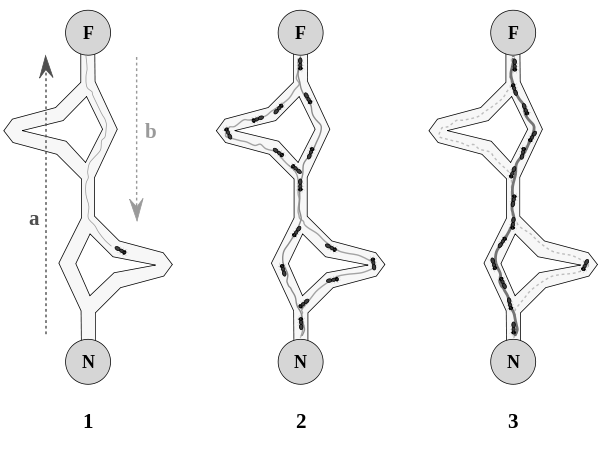
\includegraphics[width=0.5\textwidth]{pics/600px-Aco_branches.svg.png}
\caption{Работа алгоритма}
\end{wrapfigure}

В реальном мире муравьи (первоначально) ходят в случайном порядке и по нахождении продовольствия возвращаются в свою колонию, прокладывая феромонами тропы. Если другие муравьи находят такие тропы, они, вероятнее всего, пойдут по ним. Вместо того, чтобы отслеживать цепочку, они укрепляют её при возвращении, если в конечном итоге находят источник питания. Со временем феромонная тропа начинает испаряться, тем самым уменьшая свою привлекательную силу. Чем больше времени требуется для прохождения пути до цели и обратно, тем сильнее испарится феромонная тропа. На коротком пути, для сравнения, прохождение будет более быстрым, и, как следствие, плотность феромонов остаётся высокой. Испарение феромонов также имеет функцию избежания стремления к локально-оптимальному решению. Если бы феромоны не испарялись, то путь, выбранный первым, был бы самым привлекательным.

\begin{table}[h]
\caption{Сравнение генетического и муравьиного алгоритма}
\begin{tabular}{|l|ll|}
\hline
                      & \multicolumn{2}{l|}{Тесты + LTL формулы}       \\ \hline
Алгоритм              & \multicolumn{1}{l|}{Генетический} & Муравьиный \\ \hline
Среднее               & \multicolumn{1}{l|}{52405}        & 25976      \\ \hline
Сандартное отклонение & \multicolumn{1}{l|}{61440}        & 23389      \\ \hline
Медиана               & \multicolumn{1}{l|}{31507}        & 18680      \\ \hline
Минимум               & \multicolumn{1}{l|}{2875}         & 2392       \\ \hline
Максимум              & \multicolumn{1}{l|}{498365}       & 154802     \\ \hline
\end{tabular}
\end{table}

В этом случае, исследования пространственных решений были бы ограниченными. Таким образом, когда один муравей находит (например, короткий) путь от колонии до источника пищи, другие муравьи, скорее всего пойдут по этому пути, и положительные отзывы в конечном итоге приводят всех муравьёв к одному, кратчайшему, пути.
\begin{figure}
    \centering
    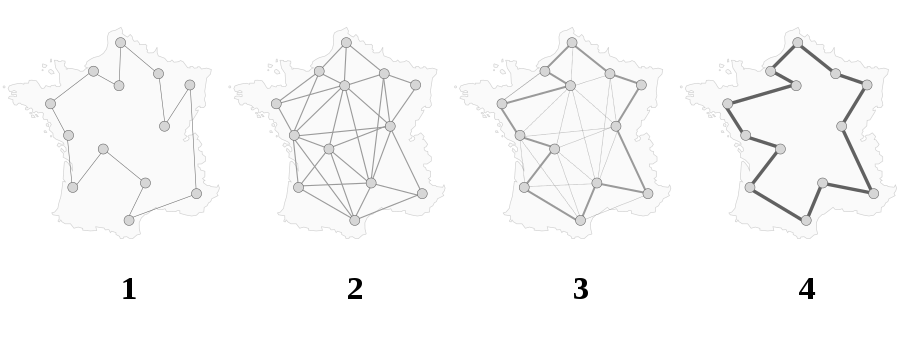
\includegraphics[scale=0.3]{pics/Без названия.png}
    \caption{Пример нахождения минимального расстояния}
\end{figure}
\section*{Вариации алгоритма}
\subsection*{Элитарная муравьиная система}
Из общего числа муравьёв выделяются так называемые «элитные муравьи». По результатам каждой итерации алгоритма производится усиление лучших маршрутов путём прохода по данным маршрутам элитных муравьёв и, таким образом, увеличение количества феромонов на данных маршрутах. В такой системе количество элитных муравьёв является дополнительным параметром, требующим определения. Так, для слишком большого числа элитных муравьёв алгоритм может «застрять» на локальных экстремумах.
\subsection*{MMAS (Max-Min муравьиная система)}

Добавляются граничные условия на количество феромонов $(T_{min},T_{max})$. Феромоны откладываются только на глобально лучших или лучших в итерации путях. Все рёбра инициализируются значением $T_{max}$.
\subsection*{Ранговая муравьиная система (ASrank)}
Все решения ранжируются по степени их пригодности. Количество откладываемых феромонов для каждого решения взвешено так, что более подходящие решения получают больше феромонов, чем менее подходящие.
\sloppypar \subsection*{Длительная ортогональная колония муравьёв (COAC)}
Механизм отложения феромонов COAC позволяет муравьям искать решения совместно и эффективно. Используя ортогональный метод, муравьи в выполнимой области могут исследовать их выбранные области быстро и эффективно, с расширенной способностью глобального поиска и точностью.
 проблем.
 \begin{lstlisting}[language=Python, caption={Муравьиный алгоритм на Python}]  
 
import numpy as np
import random as rd

def lengthCal(antPath,distmat):         
    length =[]
    dis = 0
    for i in range(len(antPath)):
        for j in range(len(antPath[i]) - 1):
            dis += distmat[antPath[i][j]]
            [antPath[i][j + 1]]
        dis += distmat[antPath[i][-1]]
        [antPath[i][0]]
        length.append(dis)
        dis = 0
    return length

distmat = np.array
([[0,35,29,67,60,50,66,44,72,41,48,97],
[35,0,34,36,28,37,55,49,78,76,70,110],
[29,34,0,58,41,63,79,68,103,69,78,130],
[67,36,58,0,26,38,61,80,87,110,100,110],
[60,28,41,26,0,61,78,73,103,100,96,130],
[50,37,63,38,61,0,16,64,50,95,81,95],
[66,55,79,61,78,16,0,49,34,82,68,83],
[44,49,68,80,73,64,49,0,35,43,30,62],
[72,78,103,87,103,50,34,35,0,47,32,48],
[41,76,69,110,100,95,82,43,47,0,26,74],
[48,70,78,100,96,81,68,30,32,26,0,58],
[97,110,130,110,130,95,83,62,48,74,58,0]])

antNum = 12                 
alpha = 1                     
beta = 3                     
pheEvaRate = 0.3           
cityNum = distmat.shape[0]
pheromone = np.ones((cityNum,cityNum))            
heuristic = 1 / (np.eye(cityNum) + distmat)
- np.eye(cityNum)      
iter,itermax = 1,100  

while iter < itermax:
    antPath = np.zeros((antNum, cityNum)).
    astype(int) - 1  
    firstCity = [i for i in range(12)]
    rd.shuffle(firstCity) 
    unvisted = []
    p = []
    pAccum = 0
    for i in range(len(antPath)):
        antPath[i][0] = firstCity[i]
    for i in range(len(antPath[0]) - 1):
        for j in range(len(antPath)):
            for k in range(cityNum):
                if k not in antPath[j]:
                    unvisted.append(k)
            for m in unvisted:
                pAccum += pheromone
                [antPath[j][i]][m] ** 
                alpha * heuristic
                [antPath[j][i]][m] ** 
                beta
            for n in unvisted:
                p.append(pheromone
                [antPath[j][i]][n] ** 
                alpha * heuristic
                [antPath[j][i]][n] **
                beta / pAccum)
            roulette = np.array(p).cumsum()
            r = rd.uniform(min(roulette), 
            max(roulette))
            for x in range(len(roulette)):
                if roulette[x] >= r: 
                    antPath[j][i + 1] = unvisted[x]
                    break
            unvisted = []
            p = []
            pAccum = 0
    pheromone = (1 - pheEvaRate) * pheromone
    length = lengthCal(antPath,distmat)
    for i in range(len(antPath)):
        for j in range(len(antPath[i]) - 1):
            pheromone[antPath[i][j]]
            [antPath[i][j + 1]] += 1 / length[i] 
        pheromone[antPath[i][-1]]
        [antPath[i][0]] += 1 / length[i]
    iter += 1
print("Shortest distance :")
print(min(length))
print("Most shortest distance :")
print(antPath[length.index(min(length))])
 
 \end{lstlisting}
 
 \begin{thebibliography}{3}
 %aaaaaaaaaaaaaaaaaaaaaaaaaaaaaaaaaaaaaaaaaaaaaaaaaaaaaaaaaaaaa
\bibitem{Ant}
Dorigo, M. Ant colony optimization / M. Dorigo. — Cambridge, Mass : MIT Press, 2004.

\bibitem{Dorigo}
Dorigo, М. Optimization, Learning and Natural Algorithms / М. Dorigo. — Rome : Politecnico di Milano, 1992.

\bibitem{Kirsanov}
Кирсанов, М. Н. Графы в Maple / М. Н. Кирсанов. — Москва : Физматлит, 2007. — 168 c.
\bibitem{Karjarov}
Кажаров, А. А. Муравьиные алгоритмы для решения транспортных задач / А. А. Кажаров // Теория и системы управления. — 2010. — Т. 1. — C. 32-45.

\end{thebibliography}
 
 %AAAAAAAAAAAAAAAAAAAAAAAAAAAAAAAAAAAAAAAAAAAAAAAAAAAAAAAAAAAA
 
 
 
 
 \begginingdouble{Быстрый обратный квадратный корень}{Уолш Г. }{example@mail.com}{Моулер К.}{example@mail.com}{быстрый приближённый алгоритм вычисления обратного квадратного корня$y=\frac{1}{\sqrt{x}}$ для положительных 32-битных}{квадратный корень, трёхмерная графика}
 
 Алгоритм использует целочисленные операции <<вычесть>> и <<битовый сдвиг>>, а также дробные <<вычесть>> и <<умножить>> — без медленных операций <<разделить>> и <<квадратный корень>>. Несмотря на <<хакерство>> на битовом уровне, приближение монотонно и непрерывно: близкие аргументы дают близкий результат. Точности (менее $0,2 \%$ в меньшую сторону и никогда — в большую) не хватает для настоящих численных расчётов, однако вполне достаточно для трёхмерной графики.
 
   \begin{figure}[h]
    \centering
    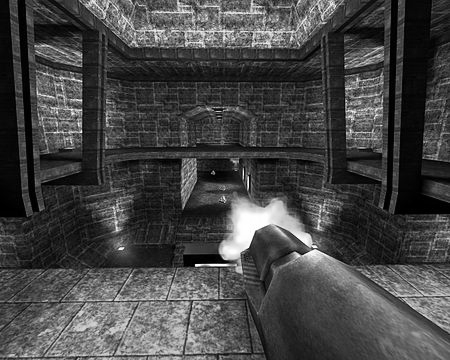
\includegraphics[scale=0.4]{pics/450px-OpenArena-Rocket.png}
    \caption{При расчёте освещения OpenArena  вычисляет углы падения и отражения через быстрый обратный квадратный корень. }
\end{figure}
 
 \section*{Алгоритм}
 

 
 Алгоритм принимает 32-битное число с плавающей запятой (одинарной точности в формате IEEE 754) в качестве исходных данных и производит над ним следующие операции:
 \begin{enumerate}
     \item Трактуя 32-битное дробное число как целое, провести операцию $y0 = 5F3759DF_{16}$ - $(x >> 1)$, где $>>$ — битовый сдвиг вправо. Результат снова трактуется как 32-битное дробное число.
     \item Для уточнения можно провести одну итерацию метода Ньютона: $y1 = y0(1,5 - 0,5xy_{0^{2}})$.
 \end{enumerate}
  \begin{lstlisting}[language=C, caption={Реализация на языке С}]  
 float Q_rsqrt( float number )
{	
	const float x2 = number * 0.5F;
	const float threehalfs = 1.5F;
	union {
		float f;
		uint32_t i;
	} conv = {number};.
	conv.i = 0x5f3759df - ( conv.i >> 1 );
	conv.f *= threehalfs - x2 * conv.f * conv.f;
	return conv.f;}
 \end{lstlisting}
 
 Реализация из Quake III: Arena считает, что $float$ по длине равен $long$, и использует для преобразования указатели (может ошибочно сработать оптимизация <<если изменился $float$, ни один $long$ не менялся>>; на GCC при компиляции в «выпуск» срабатывает предупреждение).
 \section*{Анализ и погрешность}
 
Имеем дело только с положительными числами (знаковый бит равен нулю), не денормализованными, не $\infty$ и не $NaN$. Такие числа в стандартном виде записываются как $1,mmmm_{2}·2^{e}$. Часть $1,mmmm$ называется мантиссой, $e$~—~порядком. Головную единицу не хранят (неявная единица), так что величину $0,mmmm$ назовём явной частью мантиссы. Кроме того, у машинных дробных чисел смещённый порядок: 20 записывается как $011.1111.1_{2}$.

 На положительных числах биекция <<дробное $\leftrightarrow$ целое>> (ниже обозначенная как $I_{x}$) непрерывна как кусочно-линейная функция и монотонна. Отсюда сразу же можно заявить, что быстрый обратный корень, как комбинация непрерывных функций, непрерывен. А первая его часть --- сдвиг-вычитание — к тому же монотонна и кусочно-линейна. Биекция сложна, но почти <<бесплатна>>: в зависимости от архитектуры процессора и соглашений вызова, нужно или ничего не делать, или переместить число из дробного регистра в целочисленный.
  \begin{figure}
    \centering
    \includegraphics[scale =0.3]{pics/495px-Fast_inverse_square_root_log2(1+x)_≈_x+sigma.svg.png}
    \caption{$\log_{2}(1+m_{x})\approx m_{x}+\sigma$. Приведены крайние случаи---$\sigma=0$ и $0,086$}
\end{figure}
 Например, двоичное представление 16-ричного целого числа $0x5F3759DF$ есть $0|101.1111.0|011.0111.0101.1001.1101.1111_{2}$ (Точки — границы полубайтов, вертикальные линии — границы полей компьютерного дробного). Порядок $101 1111 0_{2}$ равен $190_{10}$, после вычитания смещения $127_{10}$ получаем показатель степени $63_{10}$. Явная часть мантиссы $01 101 110 101 100 111 011 111_{2}$ после добавления неявной ведущей единицы превращается в $1,011 011 101 011 001 110 111 11_{2} = 1,432 430 148\ldots_{10}$. С учётом реальной точности компьютерных дробных $0x5F3759DF \leftrightarrow 1,432430110·2^{63}.$
 
 Обозначим $m_{x}\in [0,1)$ явную часть мантиссы числа $x, e_{x}\in \mathbb {Z}$ --- несмещённый порядок, $L=2^{23}$ — разрядность мантиссы, $ B=127$ --- смещение порядка. Число $x\equiv 2^{e_{x}}(1+m_{x})$, записанное в линейно-логарифмической разрядной сетке компьютерных дробных, можно приблизить логарифмической сеткой как $x\equiv e_{x}+\log_{2}(1+m_{2})\approx e_{x}+m_{x}+\sigma $где $\sigma$  --- параметр, используемый для настройки точности приближения. Этот параметр варьируется от 0 (формула точна при $m_{x}=0$ и $1$) до 0,086 (точна в одной точке, $m_{x}=0{,}443$).

Воспользовавшись этим приближением, целочисленное представление числа $x$ можно приблизить как


$$ I_{x}\equiv L(e_{x}+B+m_{x})\approx L\log _{2}x+L(B-\sigma )$$
Соответственно ${\log _{2}x\approx {\frac {I_{x}}{L}}-(B-\sigma )}$.

Проделаем это же для $y=\tfrac {1}{\sqrt {x}}$ (соответственно $\log _{2}y=-{\tfrac {1}{2}}\log _{2}x$), и получим

$$I_{y}\approx {\dfrac {3}{2}}L(B-\sigma )-{\dfrac {1}{2}}I_{x}$$
$$y\approx I^{-1}\left[{\dfrac {3}{2}}L(B-\sigma )-{\tfrac {1}{2}}I_{x}\right]$$
Магическая константа $\dfrac{3}{2}L(B-\sigma)$, с учётом границ $\sigma$, в арифметике дробных чисел имеет вид $c\cdot 2^{63}$, где $ c=1,5-1,5\sigma \in (1,37;1,5)$, а в двоичной записи --- $0|101.1111.0|01_{1}\ldots$ (Маленькая единица крайне вероятна, но не гарантирована нашими прикидочными расчётами.)



Можно вычислить, чему равняется первое кусочно-линейное приближение (в источнике используется не сама мантисса, а её явная часть $ t=c-1$):
\begin{itemize}
    \item Для $x\in [0,5;c-0,5): y_{01}=-x+t+\dfrac{3}{2}=-x+c+\dfrac{1}{2}$;
    \item Для $x\in [c-0,5;1): y+{02}=-\dfrac{1}{2}x+\dfrac{1}{2}t+\dfrac{5}{4}=-\dfrac{1}{2}x+\dfrac{1}{2}c+\dfrac{3}{4}$;
    \item Для $x\in [1:2): y_{03}=-\dfrac{1}{4}x+\dfrac{1}{2}t+1=-\dfrac{1}{4}+\dfrac{1}{2}c+\dfrac{1}{2}$
\end{itemize}
На больших или меньших $x$ результат пропорционально меняется: при учетверении $x$ результат уменьшается ровно вдвое.
Метод Ньютона даёт $f(y)=\dfrac{1}{y^{2}}-x,f^{'}(y)=-\dfrac{2}{y^{3}}$, и $y_{n+1}=y_{n}-\dfrac{f(y_n)}{f^{'}(y_n)}=\dfrac{y_{n}(3-xy^{2}_{n})}{2}=y_{n}(1,5-0,5)$. Функция $f(y)$ убывает и выпукла вниз, на таких функциях метод Ньютона подбирается к истинному значению слева — потому алгоритм всегда занижает ответ.
Неизвестно, откуда взялась константа $0x5F3759DF \leftrightarrow 1,4324301·2^{63}$.

 \begin{figure}
    \centering
    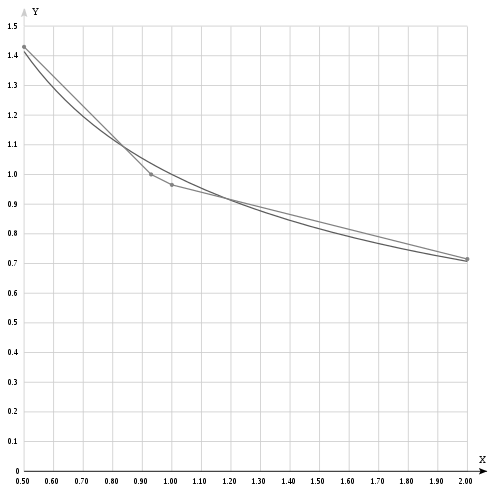
\includegraphics[scale=0.3]{pics/495px-Fast_inverse_square_root_linear_approximation.svg.png}
    \caption{Первое (кусочно-линейное) приближение быстрого обратного квадратного корня $(c = 1,43)$}
\end{figure}


 Перебором Крис Ломонт и Мэттью Робертсон выяснили, что наилучшая по предельной относительной погрешности константа для $float$ --- $0x5F375A86 \leftrightarrow 1,4324500·2^{63}$, для $double$ --- $0x5FE6EB50C7B537A9$. Правда, для double алгоритм бессмысленный (не даёт выигрыша в точности по сравнению с $float$). Константу Ломонта удалось получить и аналитически ($c = 1,432450084790142642179$), но расчёты довольно сложны. Эта цифра округляется до $1,4324500$, потому что единица младшего разряда равняется $1,19·10^{-7}$, и следующее число округляется до $1,4324502$.



После одного шага метода Ньютона результат получается довольно точный $(+0\% -0,18\%)$, что для целей компьютерной графики более чем подходит $(1⁄256 \approx 0,39\%)$. Такая погрешность сохраняется на всём диапазоне нормированных дробных чисел. Два шага дают точность в 5 цифр, после четырёх достигается погрешность $double$.

Метод Ньютона не гарантирует монотонности, но компьютерный перебор показывает, что монотонность всё-таки есть.

\begin{thebibliography}{5}
\bibitem{sommerwill}Соммервил И. Инженерия. программного обеспечения. [Текст] : 6--е изд. / пер. с англ.; М.: Вильямс, 2002. -- 624с.

\bibitem{przybylek}Przybylek Adam. Post object-oriented paradigms in software development: a comparative analysis [Текст] // Proceedings of the 1st Workshop on Advanced in Programming Languages at International Multiconference on Computer Science and Information Technology, October 15 -- 17, 2007. Wisła, Poland. -- pp. 1009-1020.

\bibitem{bon} Bonferroni C.E. Il calcolo delle assi curazioni su gruppi di test. in Studi
Onore del Professore Salvatore Ortu Carboni. Rome, Italy, 1935. P.13-60.

\bibitem{peke}Пекельник Н. М. Замечание об одном интегральном представлении // Н. М. Пекельник, О. И. Хаустова, Н. И. Попова, И. А. Трефилова. -- Актуальные проблемы гуманитарных и естественных наук. -- 2016. -- № 2-1. -- С. 33--37. 


\bibitem{ess} Esseen C.-G. A moment inequality with an application to the central limit theorem. Scand.Aktuarietidskr. J. – 1956. – V. 3-4. – P. 160-170.

\end{thebibliography}





%AAAAAAAAAAAAAAAAAAAAAAAAAAAAAAAAAAAAAAAAAAAAAAAAAAAAAAAAAAAA




\begginingdouble{SHA-3}{Дамен Й.}{daemen.j@protonworld.com}{Раймен В.}{vincent.rilnmen@estat.kuleuven.com}{Алгоритм хеширования переменной разрядности преемки SHA-2}{Криптография, SHA}
\section*{Алгоритм}



Хеш-функции семейства $SHA-3$ построены на основе конструкции криптографической губки, в которой данные сначала «впитываются» в губку, при котором исходное сообщение $M$ подвергается многораундовым перестановкам $f$, затем результат $Z$ <<отжимается>> из губки. На этапе <<впитывания>> блоки сообщения суммируются по модулю 2 с подмножеством состояния, после чего всё состояние

 \begin{figure}[h]
    \centering
    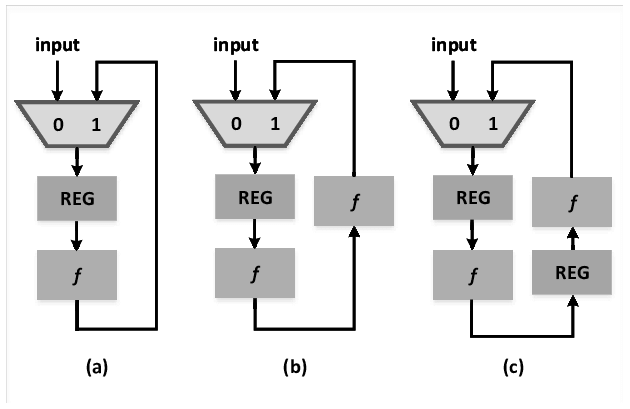
\includegraphics[scale=0.3]{pics/Architecture-of-SHA-3-Hash-Function-a-Basic-iterative-b-Unrolling-k2-c-Unrolling.png}
    \caption{Архитектура SHA-3}
\end{figure}

преобразуется с помощью функции перестановки $f$. На этапе «отжимания» выходные блоки считываются из одного и того же подмножества состояния, изменённого функцией перестановок $f$. Размер части состояния, который записывается и считывается, называется <<скоростью>> и обозначается $r$, а размер части, которая нетронута вводом / выводом, называется <<ёмкостью>> и обозначается $c$.





Алгоритм получения значения хеш-функции можно разделить на несколько этапов:
\begin{itemize}
    \item Исходное сообщение $M$ дополняется до строки $P$ длины, кратной $r$, с помощью функции дополнения (pad-функции);
    \item Строка $P$ делится на $n$ блоков длины $r$: $P_{0},P_{1},\ldots,P_{n-1}$;
    \item <<Впитывание>>: каждый блок $P_{i}$ дополняется нулями до строки длины $b$ бит и суммируется по модулю 2 со строкой состояния $S$, где $S$ --- строка длины $b$ бит ($b$ = $r$ + $c$). Перед началом работы функции все элементы $S$ равны нулю. Для каждого следующего блока состояние --- строка, полученная применением функции перестановок $f$ к результату предыдущего шага;
    \item  <<Отжимание>>: пока длина $Z$ меньше $d$ ($d$ — количество бит в результате хеш-функции), к $Z$ добавляется $r$ первых бит состояния $S$, после каждого прибавления к $S$ применяется функция перестановок $f$. Затем $Z$ обрезается до длины $d$ бит;
    \item Строка $Z$ длины $d$ бит возвращается в качестве результата.
\end{itemize}


Благодаря тому, что состояние содержит $c$ дополнительных бит, алгоритм устойчив к атаке удлинением сообщения, к которой восприимчивы алгоритмы $SHA-1$ и $SHA-2$.



В $SHA-3$ состояние $S$ --- это массив $5 × 5$ слов длиной $w = 64$ бита, всего $5 × 5 × 64 = 1600$ бит. Также в Keccak могут использоваться длины $w$, равные меньшим степеням 2 (от $w = 1$ до $w = 32$).
\section*{Дополнение}

 \begin{wrapfigure}{l}{7cm}[h]
    \centering
    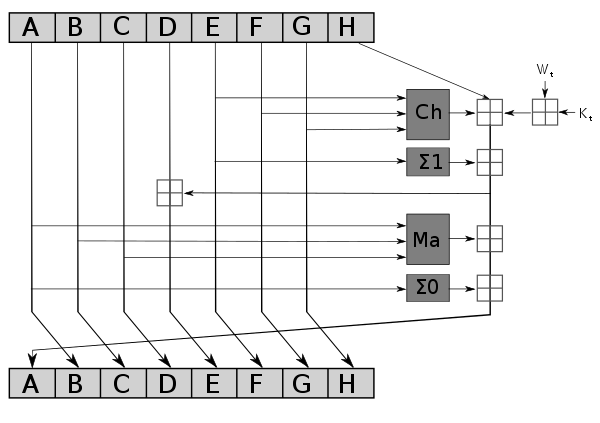
\includegraphics[scale=0.25]{pics/600px-SHA-2.svg.png}
    \caption{Схема итерации алгоритма SHA-2}
\end{wrapfigure}

Для того, чтобы исходное сообщение M можно было разделить на блоки длины $r$, необходимо дополнение. В $SHA-3$ используется паттерн $pad10*1$: к сообщению добавляется 1, после него --- 0 или больше нулевых битов (до $r-1$), в конце --- 1.

$r-1$ нулевых битов может быть добавлено, когда последний блок сообщения имеет длину $r-1$ бит. Этот блок дополняется единицей, следующий блок будет состоять из $r-1$ нулей и единицы.



Два единичных бита добавляются и в том случае, если длина исходного сообщения $M$ делится на $r$. В этом случае к сообщению добавляется блок, начинающийся и оканчивающийся единицами, между которыми $r-2$ нулевых битов. Это необходимо для того, чтобы для сообщения, оканчивающегося последовательностью битов как в функции дополнения, и для сообщения без этих битов значения хеш-функции были различны.





Первый единичный бит необходим для того, чтобы результаты хеш-функции от сообщений, различающихся несколькими нулевыми битами в конце, были различны.



\section*{Функция перестановок}

Функция перестановок, используемая в $SHA-3$, включает в себя исключающее <<ИЛИ>> (XOR), побитовое <<И>> (AND) и побитовое отрицание (NOT). Функция определена для строк длины-степени 2 $w=2^{l}$. В основной реализации $SHA-3$ $w=64$ ($l=6$).

 \begin{figure}[h]
    \centering
    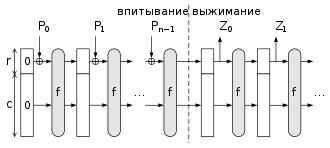
\includegraphics[scale=0.5]{pics/langru-330px-SpongeConstruction.svg (1).png}
     \caption{Конструкция функции губки, использованная в хеш-функции.}
\end{figure}

Состояние $S$ можно представить в виде трёхмерного массива $A$ размером $5 × 5 × w$. Тогда элемент массива $A[i][j][k]$ - это $(5i+j) x w+k$ бит строки состояния $S$.

Функция содержит несколько шагов: $\theta, \rho, \pi, \chi, \iota$, которые выполняются несколько раундов. На каждом шаге обозначим входной массив A, выходной массив $A^{'}$.
\subsection*{Шаг $\theta$}

Для всех $i$ и $k$, таких, что $0\leqslant i<5$, $0\leqslant k<w$, положим

$C(i,k)=A[i,0,k]\oplus A[i,1,k]\oplus A[i,2,k]\oplus A[i,3,k]\oplus A[i,4,k]$

$D(i,k)=C[(i-1){\mod 5},k]\oplus C[(i+1){\mod 5},(k-1){\bmod w}]$

Для всех $(i,j,k)$, таких, что $0\leqslant i<5$, $0\leqslant j<5$, $0\leqslant k<w$,

$A^{'}[i,j,k]=A[i,j,k]\oplus D[i,k]$
\subsection*{Шаг $\rho$}
Для всех $k$, таких, что $0\leqslant k<w$, $A^{'}[0,0,k]=A[0,0,k]$

Пусть в начале $(i,j)=(1,0)$. Для $t$ от 0 до 23:
\begin{enumerate}
    \item Для всех $k$, таких, что $0\leqslant k<w$, $A^{'}[i,j,k]=A[i,j,(k-(t+1){(t+2)/2)}{\bmod {w}}]$
    \item $(i,j)=(j,(2i+3j){\mod 5})$
    \end{enumerate}

\subsection*{Шаг  $\pi$}

Для всех $(i,j,k)$, таких, что $ 0\leqslant i<5$, $0\leqslant j<5$, $0\leqslant k<w$

$A'[i,j,k]=A[(i+3j){\mod5},i,k]$
\subsection*{Шаг $\chi$ }

Для всех $(i,j,k)$, таких, что $ 0\leqslant i<5$, $0\leqslant j<5$,

$A^{}[i,j,k]=A[i,j,k]\oplus ((A[(i+1){\mod 5},j,k]\oplus 1)\cdot A[(i+2){\mod 5},j,k])$
\subsection*{Шаг $\iota$}
Введем дополнительную функцию $rc(t)$, где вход — целое число $t$, а на выходе — бит.
\subsection*{Алгоритм $rc(t)$}
\begin{enumerate}
    \item Если $t{\mod 2}55=0$, то возвращается 1
    \item Пусть $R=[10000000]$
    \item Для i от 1 до $t \mod 255$:
    \begin{enumerate}
        \item $R = 0 || R$
        \item $R[0]=R[0]\oplus R[8]$
        \item $R[4]=R[4]\oplus R[8]$
        \item $R[5]=R[5]\oplus R[8]$
        \item $R[6]=R[6]\oplus R[8]$
        \item $R=Trunc_{8}[R]$
    \end{enumerate}
    \item Возвращается $R[0]$.
\end{enumerate}
\subsection*{Алгоритм $\iota (A,i_{r})$}
$i_{r}$ — номер раунда.
\begin{enumerate}
    \item Для всех $(i,j,k)$, таких, что $0\leqslant i<5$, $0\leqslant j<5$, $0\leqslant k<w$ $A'[i,j,k]=A[i,j,k]$
    \item Пусть $RC$ — массив длины $w$, заполненный нулями.
    \item Для $i$ от 0 до $l$: $RC[2^{i}-1]=rc(i+7i_{r})$
    \item Для всех $k$, таких, что $ 0\leqslant k<w$, $A^{'}[0,0,k]=A^{'}[0,0,k]\oplus RC[k]$
\end{enumerate}
\subsection*{Алгоритм перестановок}
\begin{enumerate}
    \item Перевод строки $S$ в массив $A$
    \itemДля $i_{r}$ от $12+2l-n_{r}$ до $12+2l-1$ $A^{'}=\iota (\chi (\pi (\rho (\theta (A)))),i_{r})$
    \item  Перевод массива $A^{'}$ в строку $S^{'}$ длины $b$
\end{enumerate}

\section*{Настройки}
Оригинальный алгоритм Keccak имеет множество настраиваемых параметров с целью обеспечения оптимального соотношения криптостойкости и быстродействия для определённого применения алгоритма на определённой платформе. Настраиваемыми величинами являются: размер блока данных, размер состояния алгоритма, количество раундов в функции $f()$ и другие.

\begin{table}[h]
\caption{Параметры типов SHA-3}
    \centering
    
    \begin{tabular}{|c|c|c|c|}
    \hline
         Тип & Длинна вывода & Частота & Объём  \\ \hline
         $SHA-3$-224& 224 & 1152 & 448  \\ \hline
         $SHA-3$-256& 256 & 1088 & 512  \\ \hline
         $SHA-3$-384& 384 & 832 & 768  \\ \hline
         $SHA-3$-512& 512 &576 & 1024  \\ \hline
    \end{tabular}
    
    \label{tab:my_label}
\end{table}


На протяжения конкурса хеширования Национального института стандартов и технологий участники имели право настраивать свои алгоритмы для решения возникших проблем. Так, были внесены некоторые изменения в Keccak: количество раундов было увеличено с 18 до 24 с целью увеличения запаса безопасности.

Авторы Keccak учредили ряд призов за достижения в криптоанализе данного алгоритма.

\begin{table}
\caption{Соответсвие параметров между SHA-3 и Keccak}
\begin{tabular}{|l|l|}

\hline
Функции       & Формулы                    \\ \hline
SHA-224(M)    & KECCAK{[}448{]}(M||01,224) \\ \hline
SHA3-256(M)   & KECCAK{[}512{]}(M||01,256) \\ \hline
SHA3-384(M)   & KECCAK{[}768{]}(M||01,384) \\ \hline
SHA3-512(M)   & KECCAK{[}1024{]}(M||01,512)\\ \hline
SHAKE128(M,d) & KECCAK{[}256{]}(M||1111,d) \\ \hline
SHAKE256(M,d) & KECCAK{[}512{]}(M||1111,d) \\ \hline
\end{tabular}

\end{table}

Версия алгоритма, принятая в качестве окончательного стандарта $SHA-3$, имеет несколько незначительных отличий от оригинального предложения Keccak на конкурс. В частности, были ограничены некоторые параметры (отброшены медленные режимы $c=768$ и $c=1024$), в том числе для увеличения производительности. Также в стандарте были введены <<функции с удлиняемым результатом>> (XOF, Extendable Output Functions) $SHAKE128$ и $SHAKE256$, для чего хешируемое сообщение стало необходимо дополнять <<суффиксом>> из 2 или 4 бит, в зависимости от типа функции.


\section*{Криптоанализ}
\begin{center}
\begin{longtable}{|p{2.1cm}|p{2.1cm}|p{1.1cm}|p{1.4cm}|p{1.3cm}|}
\caption{Результаты криптоанализа}\\
\hline
\textbf{Цель} & \textbf{Тип атаки} & \textbf{Выход} & \textbf{Вариант} & \textbf{CF Call} \\
\hline
\endfirsthead
\multicolumn{4}{c}%
{\tablename\ \thetable\ -- \textit{Продолжение таблицы \thetable }} \\
\hline
\textbf{Цель} & \textbf{Тип атаки} & \textbf{Выход} & \textbf{Вариант} & \textbf{CF Call} \\
\hline
\endhead
\hline \multicolumn{4}{r}{\textit{На следующей странице}} \\
\endfoot
\hline
\endlastfoot
Хеш-функция  & Коллизия                     & 160      & 1, 2 раунда & \\ \hline
Хеш-функция  & Нахождение прообраза         & 80       & 1, 2 раунда & \\ \hline
Перестановки & Атака-различитель            & Все      &  24 раунда &$ 2^{1579}$ \\\hline
Перестановки & Диффере\-нциальное свойство    & Все      &  8 раундов &$2^{491.47}$ \\ \hline
Хеш-функция  & Атака-различитель            & 224, 256 & 4 раунда &$2^{25}$ \\\hline
Хеш-функция  & Коллизия                     & 224, 256 & 2 раунда &$2^{33}$ \\\hline
Хеш-функция  & Нахождение второго прообраза &224, 256  & 2 раунда &$2^{33}$ \\\hline
Хеш-функция  & Нахождение второго прообраза & 512      & 6 раундов& $2^{506}$\\ \hline
Хеш-функция  & Нахождение второго прообраза & 512      & 7 раундов & $2^{507}$\\\hline
Хеш-функция  & Нахождение второго прообраза & 512      & 8 раундов & $2^{511.5}$ \\ \hline
Хеш-функция  & Коллизия                     & 224, 256 & 4 раунда & \\ \hline
\end{longtable}
\end{center}



\begin{thebibliography}{3}
\bibitem{sommerwill}Соммервил И. Инженерия. программного обеспечения. [Текст] : 6--е изд. / пер. с англ.; М.: Вильямс, 2002. -- 624с.

\bibitem{przybylek}Przybylek Adam. Post object-oriented paradigms in software development: a comparative analysis [Текст] // Proceedings of the 1st Workshop on Advanced in Programming Languages at International Multiconference on Computer Science and Information Technology, October 15 -- 17, 2007. Wisła, Poland. -- pp. 1009-1020.

\bibitem{bon} Bonferroni C.E. Il calcolo delle assi curazioni su gruppi di test. in Studi
Onore del Professore Salvatore Ortu Carboni. Rome, Italy, 1935. P.13-60.

\end{thebibliography}
\newpage \null
\renewcommand\indexname{Авторский указатель}
\printindex \thispagestyle{empty}

\newpage\thispagestyle{empty}

    \begin{center}
    %\textsc{\textbf{}}
    \vspace{15cm}
    \Large Научное издание \linebreak
    Сборник статей\\
    2022
    
    
    Дата выхода в свет: 04.05.2022. Формат 210 x 148\linebreak
    Усл. печ. л. 16. Тираж 1 экз. Цена 0 руб. Заказ 1
    \thispagestyle{empty}
    \end{center}
    
\end{document}
